\documentclass{ximera}

 

\usepackage{epsfig}

\graphicspath{
  {./}
  {figures/}
}

\usepackage{morewrites}
\makeatletter
\newcommand\subfile[1]{%
\renewcommand{\input}[1]{}%
\begingroup\skip@preamble\otherinput{#1}\endgroup\par\vspace{\topsep}
\let\input\otherinput}
\makeatother

\newcommand{\includeexercises}{\directlua{dofile("/home/jim/linearAlgebra/laode/exercises.lua")}}

%\newcounter{ccounter}
%\setcounter{ccounter}{1}
%\newcommand{\Chapter}[1]{\setcounter{chapter}{\arabic{ccounter}}\chapter{#1}\addtocounter{ccounter}{1}}

%\newcommand{\section}[1]{\section{#1}\setcounter{thm}{0}\setcounter{equation}{0}}

%\renewcommand{\theequation}{\arabic{chapter}.\arabic{section}.\arabic{equation}}
%\renewcommand{\thefigure}{\arabic{chapter}.\arabic{figure}}
%\renewcommand{\thetable}{\arabic{chapter}.\arabic{table}}

%\newcommand{\Sec}[2]{\section{#1}\markright{\arabic{ccounter}.\arabic{section}.#2}\setcounter{equation}{0}\setcounter{thm}{0}\setcounter{figure}{0}}

\newcommand{\Sec}[2]{\section{#1}}

\setcounter{secnumdepth}{2}
%\setcounter{secnumdepth}{1} 

%\newcounter{THM}
%\renewcommand{\theTHM}{\arabic{chapter}.\arabic{section}}

\newcommand{\trademark}{{R\!\!\!\!\!\bigcirc}}
%\newtheorem{exercise}{}

\newcommand{\dfield}{{\sf dfield9}}
\newcommand{\pplane}{{\sf pplane9}}

\newcommand{\EXER}{\section*{Exercises}}%\vspace*{0.2in}\hrule\small\setcounter{exercise}{0}}
\newcommand{\CEXER}{}%\vspace{0.08in}\begin{center}Computer Exercises\end{center}}
\newcommand{\TEXER}{} %\vspace{0.08in}\begin{center}Hand Exercises\end{center}}
\newcommand{\AEXER}{} %\vspace{0.08in}\begin{center}Hand Exercises\end{center}}

% BADBAD: \newcommand{\Bbb}{\bf}

\newcommand{\R}{\mbox{$\Bbb{R}$}}
\newcommand{\C}{\mbox{$\Bbb{C}$}}
\newcommand{\Z}{\mbox{$\Bbb{Z}$}}
\newcommand{\N}{\mbox{$\Bbb{N}$}}
\newcommand{\D}{\mbox{{\bf D}}}
\usepackage{amssymb}
%\newcommand{\qed}{\hfill\mbox{\raggedright$\square$} \vspace{1ex}}
%\newcommand{\proof}{\noindent {\bf Proof:} \hspace{0.1in}}

\newcommand{\setmin}{\;\mbox{--}\;}
\newcommand{\Matlab}{{M\small{AT\-LAB}} }
\newcommand{\Matlabp}{{M\small{AT\-LAB}}}
\newcommand{\computer}{\Matlab Instructions}
\newcommand{\half}{\mbox{$\frac{1}{2}$}}
\newcommand{\compose}{\raisebox{.15ex}{\mbox{{\scriptsize$\circ$}}}}
\newcommand{\AND}{\quad\mbox{and}\quad}
\newcommand{\vect}[2]{\left(\begin{array}{c} #1_1 \\ \vdots \\
 #1_{#2}\end{array}\right)}
\newcommand{\mattwo}[4]{\left(\begin{array}{rr} #1 & #2\\ #3
&#4\end{array}\right)}
\newcommand{\mattwoc}[4]{\left(\begin{array}{cc} #1 & #2\\ #3
&#4\end{array}\right)}
\newcommand{\vectwo}[2]{\left(\begin{array}{r} #1 \\ #2\end{array}\right)}
\newcommand{\vectwoc}[2]{\left(\begin{array}{c} #1 \\ #2\end{array}\right)}

\newcommand{\ignore}[1]{}


\newcommand{\inv}{^{-1}}
\newcommand{\CC}{{\cal C}}
\newcommand{\CCone}{\CC^1}
\newcommand{\Span}{{\rm span}}
\newcommand{\rank}{{\rm rank}}
\newcommand{\trace}{{\rm tr}}
\newcommand{\RE}{{\rm Re}}
\newcommand{\IM}{{\rm Im}}
\newcommand{\nulls}{{\rm null\;space}}

\newcommand{\dps}{\displaystyle}
\newcommand{\arraystart}{\renewcommand{\arraystretch}{1.8}}
\newcommand{\arrayfinish}{\renewcommand{\arraystretch}{1.2}}
\newcommand{\Start}[1]{\vspace{0.08in}\noindent {\bf Section~\ref{#1}}}
\newcommand{\exer}[1]{\noindent {\bf \ref{#1}}}
\newcommand{\ans}{}
\newcommand{\matthree}[9]{\left(\begin{array}{rrr} #1 & #2 & #3 \\ #4 & #5 & #6
\\ #7 & #8 & #9\end{array}\right)}
\newcommand{\cvectwo}[2]{\left(\begin{array}{c} #1 \\ #2\end{array}\right)}
\newcommand{\cmatthree}[9]{\left(\begin{array}{ccc} #1 & #2 & #3 \\ #4 & #5 &
#6 \\ #7 & #8 & #9\end{array}\right)}
\newcommand{\vecthree}[3]{\left(\begin{array}{r} #1 \\ #2 \\
#3\end{array}\right)}
\newcommand{\cvecthree}[3]{\left(\begin{array}{c} #1 \\ #2 \\
#3\end{array}\right)}
\newcommand{\cmattwo}[4]{\left(\begin{array}{cc} #1 & #2\\ #3
&#4\end{array}\right)}

\newcommand{\Matrix}[1]{\ensuremath{\left(\begin{array}{rrrrrrrrrrrrrrrrrr} #1 \end{array}\right)}}

\newcommand{\Matrixc}[1]{\ensuremath{\left(\begin{array}{cccccccccccc} #1 \end{array}\right)}}



\renewcommand{\labelenumi}{\theenumi)}
\newenvironment{enumeratea}%
{\begingroup
 \renewcommand{\theenumi}{\alph{enumi}}
 \renewcommand{\labelenumi}{(\theenumi)}
 \begin{enumerate}}
 {\end{enumerate}\endgroup}



\newcounter{help}
\renewcommand{\thehelp}{\thesection.\arabic{equation}}

%\newenvironment{equation*}%
%{\renewcommand\endequation{\eqno (\theequation)* $$}%
%   \begin{equation}}%
%   {\end{equation}\renewcommand\endequation{\eqno \@eqnnum
%$$\global\@ignoretrue}}

%\input{psfig.tex}

\author{Martin Golubitsky and Michael Dellnitz}

%\newenvironment{matlabEquation}%
%{\renewcommand\endequation{\eqno (\theequation*) $$}%
%   \begin{equation}}%
%   {\end{equation}\renewcommand\endequation{\eqno \@eqnnum
% $$\global\@ignoretrue}}

\newcommand{\soln}{\textbf{Solution:} }
\newcommand{\exercap}[1]{\centerline{Figure~\ref{#1}}}
\newcommand{\exercaptwo}[1]{\centerline{Figure~\ref{#1}a\hspace{2.1in}
Figure~\ref{#1}b}}
\newcommand{\exercapthree}[1]{\centerline{Figure~\ref{#1}a\hspace{1.2in}
Figure~\ref{#1}b\hspace{1.2in}Figure~\ref{#1}c}}
\newcommand{\para}{\hspace{0.4in}}

\renewenvironment{solution}{\suppress}{\endsuppress}

\ifxake
\newenvironment{matlabEquation}{\begin{equation}}{\end{equation}}
\else
\newenvironment{matlabEquation}%
{\let\oldtheequation\theequation\renewcommand{\theequation}{\oldtheequation*}\begin{equation}}%
  {\end{equation}\let\theequation\oldtheequation}
\fi

\makeatother


\title{Laplace Transforms and Their Computation}

\begin{document}
\begin{abstract}
\end{abstract}
\maketitle

 \label{S:13.3}
\index{Laplace transform!existence}

This section divides into three parts.  In the first part, we give an explicit 
formula for the Laplace transform and verify that this formula satisfies 
properties \eqref{Tprops}.  In the second part, we compute a table of Laplace
transforms for a number of special functions including step functions and
impulse functions.  In the third part we discuss two properties of Laplace
transforms that are useful when computing inverse Laplace transforms of
functions of the type that appear when solving forced second order equations.

\begin{definition}  \label{D:laplace}
Let $x(t)$ be a function that is defined for $0\le t < \infty$.
Then the function ${\cal L}[x](s)$ is defined by
\begin{equation} \label{E:laplace}
{\cal L}[x](s) = \int_0^{\infty} e^{-st} x(t)\; dt
\end{equation}
and is called the {\em Laplace transform\/} of $x(t)$.
\end{definition}\index{Laplace transform!definition}

Note that the Laplace transform is an improper 
integral --- which implies that some care must be taken when discussing 
its properties.  Indeed, for some functions the Laplace transform does 
not exist for all values of $s$.  What usually happens is that 
the Laplace transform exists for all values of $s$ larger than some 
number $a$.  As an example, we compute \eqref{eq:Lexp} directly using 
Definition~\ref{D:laplace}.  Let $x(t)=e^{at}$ and compute 
\begin{equation}  \label{e:expat}
{\cal L}[x](s) = \int_0^{\infty} e^{(a-s)t}\; dt=
\lim\limits_{h\to \infty} \frac{1}{s-a}\left( 1-e^{(a-s)h} \right)
=\left\{ \begin{array}{cl} \frac{\dps 1}{\dps s-a} & \mbox{for $s>a$,}\\
\infty & \mbox{for $s\le a$.}\end{array}\right.
\end{equation}

\subsubsection*{The Laplace Transform is Linear}
\index{Laplace transform!linearity}

The first step in verifying properties \eqref{Tprops} is to show that the 
Laplace transform ${\cal L}$ is linear, that is, to 
show that \eqref{Tprops}(a) holds.
\begin{proposition}  \label{prop:linLap}
Suppose $x(t)$ and $y(t)$ are functions for which the Laplace transforms
${\cal L}[x](s)$, ${\cal L}[y](s)$ exist for $s>a$, and let $c$ be real. 
Then for all $s>a$
\begin{equation}  \label{eq:linLap}
\begin{array}{rcl}
{\cal L}[x + y] &  = & {\cal L}[x] + {\cal L}[y] \\
{\cal L}[cx] & = & c{\cal L}[x].
\end{array}
\end{equation}
\end{proposition}

\begin{proof} Using properties of integrals we obtain for each $s>a$
\begin{eqnarray*}
{\cal L}[x+y](s) &=& \int_0^{\infty} e^{-st} (x(t)+y(t))\; dt\\
&=& \int_0^{\infty} e^{-st} x(t)\; dt + \int_0^{\infty} e^{-st} y(t)\; dt\\
&=& {\cal L}[x](s)+ {\cal L}[y](s).
\end{eqnarray*}
A similar computation verifies that ${\cal L}$ commutes with scalar 
multiplication.  \end{proof}

\subsubsection*{The Derivative Property of Laplace Transforms is Valid}
\index{Laplace transform!derivative property}

Next we verify the important derivative property \eqref{Tprops}(c) of the 
Laplace transform.  

\begin{proposition}  \label{prop:derLap}
Suppose that $x$ is a differentiable function such that 
$|x(t)|\le Me^{at}$ for constants $a>0$ and $M>0$.  
Then
\begin{itemize}
\item[(a)] the Laplace transform ${\cal L}[x](s)$ exists for $s>a$; 
\item[(b)] ${\cal L}[\dot x](s) = s{\cal L}[x](s) - x(0) \quad 
\mbox{for $s>a$.}$
\end{itemize}
\end{proposition}

\begin{proof} 
\noindent (a) Observe that by the assumption on the growth of 
$x(t)$ we have for $s>a$
\[
\lim\limits_{h\to \infty}\left|\int_0^h e^{-st} x(t)\; dt\right|
\le \lim\limits_{h\to \infty}\int_0^h Me^{(a-s)t}\; dt
=\lim\limits_{h\to \infty}\left.\frac{Me^{(a-s)t}}{a-s}\right|_0^h
=\frac{M}{s-a}<\infty.
\]
Hence the Laplace transform ${\cal L}[x](s)$ exists for $s>a$.

\noindent(b) First note that
\[
\lim\limits_{h\to \infty} |e^{-sh} x(h)|\le
\lim\limits_{h\to \infty} |Me^{(a-s)h}| = 0.
\]
Now use the definition of improper integrals and integration by parts to 
compute 
\begin{eqnarray*}
{\cal L}[\dot x](s) &=& \int_0^{\infty} e^{-st} \dot x(t)\; dt\\
& = & \lim\limits_{h\to \infty}\int_0^h e^{-st} \dot x(t)\; dt\\
& = & \lim\limits_{h\to \infty}\left(\left.e^{-st}x(t)\right|_0^h -
\int_0^h (-s)e^{-st} x(t)\; dt\right)\\
&=& \lim\limits_{h\to \infty} \left( e^{-sh} x(h) - x(0)\right) +
s\lim\limits_{h\to \infty} \int_0^h e^{-st} x(t)\; dt\\
&=& -x(0) + s{\cal L}[x](s)
\end{eqnarray*}
for $s>a$.  \end{proof}

Finally, we remark that \eqref{Tprops}(b) is valid, but that its proof is 
beyond the scope of this course.  One method of proof is to develop an 
explicit integral formula for the inverse Laplace transform. 


\subsection*{A Table of Laplace Transforms}
\index{Laplace transform!table of}

In order to solve differential equations using the method of Laplace 
transforms, we need to have a table of Laplace transforms readily available.  
We now compute the Laplace transform for the functions in 
Table~\ref{tab:Laplist}.   These functions include the discontinuous step 
function\index{step function} 
\[
H_c(t) = \left\{\begin{array}{ll}
0 & \mbox{for $0\le t < c$}\\
1 & \mbox{for $t\ge c$}
\end{array}\right. 
\]\index{$H_c(t)$}
where $c$ is a positive constant and the hitherto undefined Dirac delta 
function $\delta_c(t)$.  See Figure~\ref{F:H1} for a graph of $H_1$.

\begin{figure}[htb]
           \centerline{%
           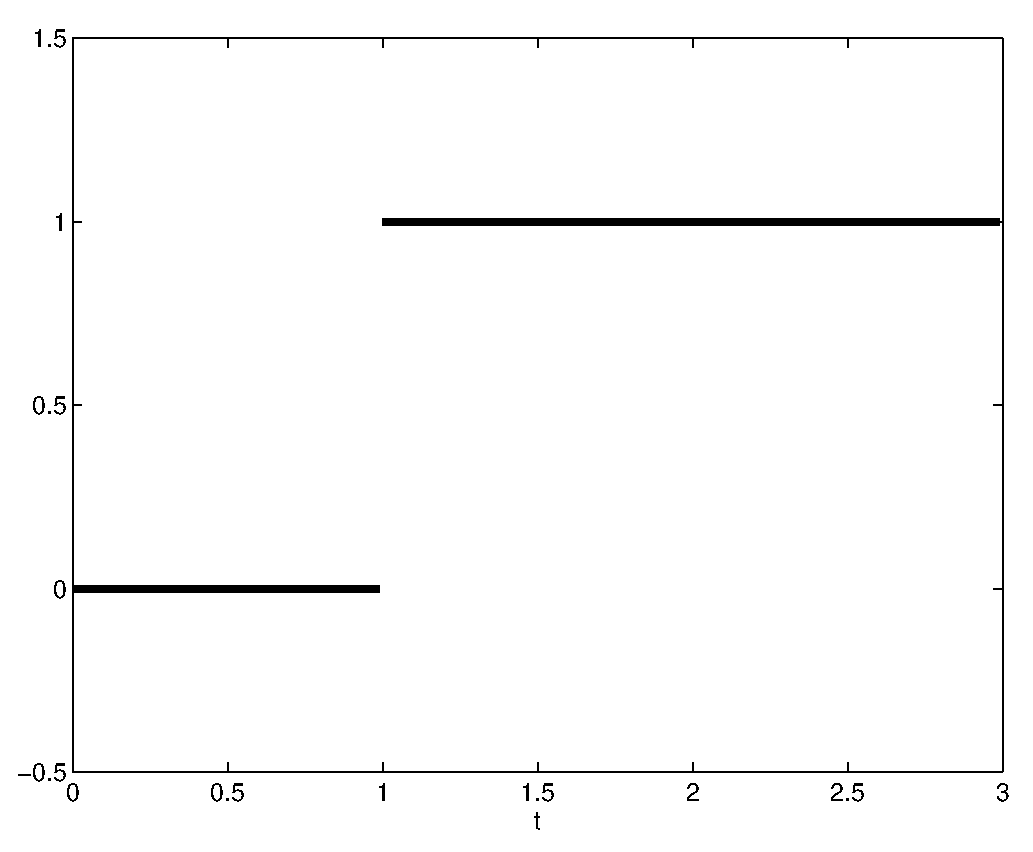
\psfig{file=../figures/H1.eps,width=2.5in}}
           \caption{Graph of $H_1(t)$.}
           \label{F:H1}
\end{figure}

We derive some of these formulas by using the Laplace transform formulas for 
derivatives \eqref{Tprops}(c) and \eqref{eq:dderLap}.  (We could compute these 
transforms directly by integration from Definition~\ref{D:laplace}, but the 
method we choose is simpler and illustrates the power of the derivative 
formulas.)  Note that we have already computed the Laplace transforms 
of the first two functions in Table~\ref{tab:Laplist} when deriving 
\eqref{eq:Lexp}.

\begin{table}[htb]
\begin{center}
\begin{tabular}{|c|c|}
\hline
Function $y(t)$ & Laplace transform ${\cal L}[y](s)$\\
\hline
$1$ & $\frac{\dps 1}{\dps s}$\\
$e^{at}$ & $\frac{\dps 1}{\dps s-a}$\\
$\cos(\tau t)$ & $\frac{\dps s}{\dps s^2 + \tau^2}$\\
$\sin(\tau t)$ & $\frac{\dps \tau}{\dps s^2 + \tau^2}$\\
$t^n$ & $\frac{\dps n!}{\dps s^{n+1}}$\\
$H_c(t)$ & $\frac{1}{\dps s}e^{-cs}$\\
$\delta_c(t)$ & $e^{-cs}$\\
\hline
\end{tabular}
\end{center}
\caption{Laplace transforms.}
\label{tab:Laplist}
\end{table}


\subsubsection*{The Laplace Transforms: ${\cal L}[\cos(\tau t)]$ and 
${\cal L}[\sin(\tau t)]$}

To compute ${\cal L}[x]$ where $x(t)=\cos(\tau t)$, observe that $x(t)$ is 
a solution to the initial value problem
\begin{eqnarray*}
\ddot{x}+\tau^2 x & = & 0\\ 
x(0) & = & 1 \\ 
\dot{x}(0) & = & 0.
\end{eqnarray*}
It follows from \eqref{eq:dderLap} that
\[
s^2{\cal L}[x] - s + \tau^2 {\cal L}[x] = 0.
\]
Hence
\[
{\cal L}[x] = \frac{s}{s^2+\tau^2},
\]
as desired.  Similarly, note that $x(t)=\sin(\tau t)$ satisfies the initial
value problem
\begin{eqnarray*}
\ddot{x}+\tau^2 x & = & 0 \\
  x(0) & = & 0 \\
 \dot{x}(0) & = & \tau.
\end{eqnarray*}
The computation of the Laplace transform for $\sin(\tau t)$ proceeds
identically as the computation of ${\cal L}[\cos(\tau t)]$.

\subsubsection*{The Laplace Transform: ${\cal L}[t^n]$}

Next, we compute ${\cal L}[t^n]$ by applying \eqref{Tprops}(c) $n$ times.
That is, 
\[
{\cal L}[t^n] = \frac{n}{s}{\cal L}[t^{n-1}] = \cdots =
\frac{n!}{s^n}{\cal L}[1] = \frac{n!}{s^{n+1}}.
\]

\subsubsection*{The Laplace Transform: ${\cal L}[H_c(t)]$}

We compute the Laplace transform of the step function $H_c(t)$ by direct 
integration.  
\[
{\cal L}[H_c](s) = \int_0^{\infty} e^{-st}H_c(t)\; dt
= \int_c^{\infty} e^{-st}\; dt
=\left\{ \begin{array}{cl} \frac{1}{\dps s}e^{-cs} & \mbox{for $s>0$,}\\
\infty & \mbox{for $s\le 0$.}\end{array}\right.
\]


\subsubsection*{The Laplace Transform of Dirac Delta Functions}
\index{Dirac delta function}

Suppose that a strong external force is applied at time $t=c$, but only for a 
very short time $h$.  Then the forcing function is approximated by
\begin{equation}  \label{eq:deltah}
\begin{array}{rcl}
g_h(t) & =  & 
\left\{\begin{array}{cc} \frac{1}{h} & c\leq t \leq c+h \\ 
		0 & \mbox{otherwise} \end{array} \right. \\
 & = & \frac{1}{h} \left(H_c(t)-H_{c+h}(t)\right). 
\end{array}
\end{equation}
The graph of $g_h$ is given in Figure~\ref{fig:deltah}.  It is not clear how 
to take the limit of $g_h(t)$ as $h\to 0$ in \eqref{eq:deltah}, since this limit 
leads to a `function' that is infinity at $c$ and zero elsewhere.  Despite 
this difficulty, the limit is called the {\em Dirac delta function}
\index{Dirac delta function} and is denoted by $\delta_c(t)$.  We compute the 
Laplace transform of the $\delta_c(t)$ by first computing the Laplace 
transform of the approximating function $g_h(t)$ and then taking the limit of 
the Laplace transforms of the approximation as $h\to 0$.

\begin{figure}[htb]
           \centerline{%
           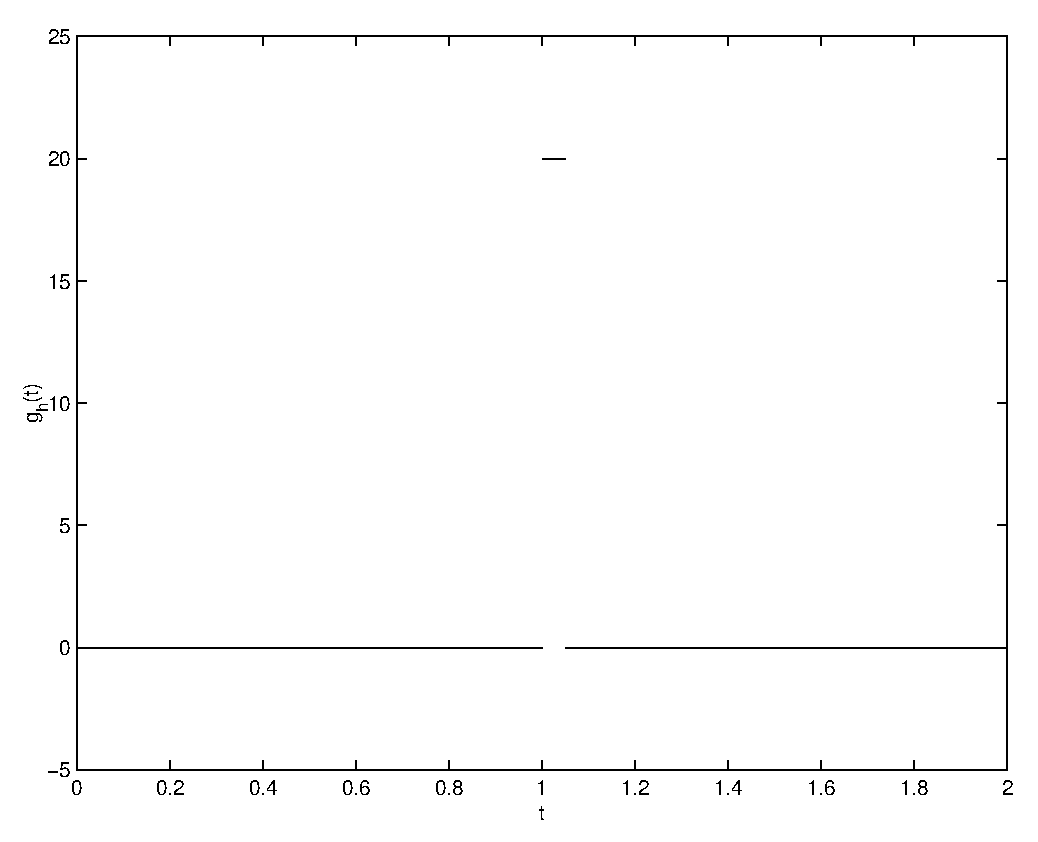
\psfig{file=../figures/deltah.eps,width=2.8in}}
           \caption{Graph of the approximating function $g_h(t)$ of  
	   \protect\eqref{eq:deltah} for $c=1$ and $h=0.05$.}
           \label{fig:deltah}
\end{figure}

The Laplace transform of the approximating function $g_h(t)$ is found using 
the linearity of ${\cal L}$ and Table~\ref{tab:Laplist}, that is,
\[
{\cal L}[g_h] =  \frac{1}{h} \left({\cal L}[H_c]-{\cal L}[H_{c+h}]\right) =
\frac{1}{h}\left(\frac{1}{s}e^{-cs}-
\frac{1}{s}e^{-(c+h)s}\right) = \frac{1}{s}e^{-cs}\frac{1-e^{-sh}}{h}.
\]
We claim that
\[
\lim_{h\to 0} \left(\frac{1-e^{-sh}}{h}\right)=s,
\]
from which it follows that 
\[
\lim_{h\to 0} {\cal L}[g_h](s)=e^{-cs}.
\]
This result justifies writing
\begin{equation}  \label{e:lapdel}
{\cal L}[\delta_c] = e^{-cs}.
\end{equation}
To verify the claim, let $f(y)=e^{-sy}$ and recall that 
\[
f'(0) = \lim_{h\to 0} \frac{f(h)-f(0)}{h} =\lim_{h\to 0} \frac{e^{-sh}-1}{h}.
\]
Since $f'(0)=-s$, it follows that
\[
\lim_{h\to 0} \left(\frac{1-e^{-sh}}{h}\right)=-f'(0)=s,
\]
as claimed.


\subsection*{Additional Techniques for Laplace Transforms}

At the end of Section~\ref{S:13.1} we showed that when solving second order
differential equations by the method of Laplace transforms, it is necessary to 
compute inverse Laplace transforms of functions like
\begin{equation}  \label{E:1sttype}
\frac{1}{(s-B)^2+C^2} \AND \frac{s-B}{(s-B)^2+C^2}
\end{equation}
and 
\begin{equation}  \label{2ndtype}
\frac{1}{(s-B)^2+C^2}G(s) \AND \frac{s-B}{(s-B)^2+C^2}G(s)
\end{equation}
where $G(s)$ is the Laplace transform of the forcing function $g(t)$.
See \eqref{e:sampleLT}.  

\subsubsection*{Inverse Laplace Transforms of Shifted Functions}

The next proposition enables us to calculate inverse Laplace transforms for
functions of type \eqref{E:1sttype}.

\begin{proposition}  \label{prop:eHcLap1}
Suppose that $Y(s)={\cal L}[y(t)](s)$ exists.  Then
\[
\begin{array}{rrcl}
\mbox{(a)} & {\cal L}[e^{at}y(t)](s) & = & Y(s-a)\\
\mbox{(b)} & {\cal L}^{-1}[Y(s-a)](t) & = & e^{at}y(t).
\end{array}
\]
\end{proposition}
\index{Laplace transform!general properties}\index{Laplace transform!inverse}

\begin{proof}  To verify (a) compute
\[
{\cal L}[e^{at}y(t)](s) = \int_0^{\infty} e^{-st}e^{at} y(t)\; dt
= \int_0^{\infty} e^{-(s-a)t} y(t)\; dt = {\cal L}[y(t)](s-a) = Y(s-a).
\]
Part (b) follows by applying the inverse Laplace transform to both sides 
of (a).  \end{proof}

For example, suppose that we want to compute the inverse Laplace transform of 
\begin{equation}  \label{e:exlappf}
\frac{s-1}{s^2+2s+5}.
\end{equation}
The first step in this computation is to write the denominator as the sum of 
two squares and to shift the numerator.   That is,
\begin{equation}  \label{e:pf1}
\frac{s-1}{s^2+2s+5} = \frac{(s+1)-2}{(s+1)^2+4} = 
\frac{s+1}{(s+1)^2+4} - 2\frac{1}{(s+1)^2+4}.
\end{equation}
We can now find the inverse Laplace transform of the right hand side of 
\eqref{e:pf1}.  Except for the shift of $s$ to $s+1$, the rearranged expression 
\eqref{e:pf1} is one whose inverse Laplace transform can be read from 
Table~\ref{tab:Laplist}.  More precisely, let 
\[
Y(s) = \frac{s}{s^2+4} - 2\frac{1}{s^2+4},
\]
so that the right hand side of \eqref{e:pf1} is $Y(s+1)$.  Using 
Table~\ref{tab:Laplist} the inverse Laplace transform of $Y(s)$ is
\begin{equation}  \label{e:exlappf2}
{\cal L}\inv[Y(s)](t) = 
{\cal L}\inv\left[\frac{s}{s^2+4} - 2\frac{1}{s^2+4}\right](t) = 
\cos(2t) - \sin(2t) = y(t).
\end{equation}
Using Proposition~\ref{prop:eHcLap1}(b) we can compute the inverse Laplace 
transform of $Y(s+1)$ 
as
\[
{\cal L}^{-1}[Y(s+1)](t) = e^{-t}y(t)
\]
That is,
\[
{\cal L}^{-1}\left[\frac{s-1}{s^2+2s+5}\right](t) = e^{-t}(\cos(2t)-\sin(2t)).
\]

\subsubsection*{Another Useful Property of the Laplace Transform}

Next, we examine the Laplace transform of a function that is multiplied 
by the jump function $H_c(t)$ and by doing so we will be able to compute the
inverse Laplace transform of functions like \eqref{2ndtype} when $G(s)$ is the 
Laplace transform of a discontinuous forcing function.

\begin{proposition}  \label{prop:eHcLap2}
Suppose that $Y(s)={\cal L}[y(t)](s)$ exists.  Then
\[
\begin{array}{rrcl}
\mbox{(a)} & {\cal L}[H_c(t)y(t-c)](s) & = & e^{-cs} Y(s) \\
\mbox{(b)} & {\cal L}^{-1}[e^{-cs}Y(s)](t) & = & H_c(t)y(t-c).
\end{array}
\]
\end{proposition}

\begin{proof} (a)  Compute
\[
{\cal L}[H_c(t)y(t-c)](s) = \int_0^{\infty} e^{-st}H_c(t) y(t-c)\; dt
= \int_c^{\infty} e^{-st}y(t-c)\; dt.
\]
On substituting $t+c$ for $t$ we obtain
\[
{\cal L}[H_c(t)y(t-c)](s)=\int_0^{\infty} e^{-s(t+c)}y(t)\; dt
=e^{-cs} \int_0^{\infty} e^{-st}y(t)\; dt
=e^{-cs} Y(s).
\]
Part (b) follows by applying the inverse Laplace transform to both sides 
of (a).  \end{proof}

As an application of Proposition~\ref{prop:eHcLap2}(b), we find that
\[
{\cal L}^{-1}\left[ e^{-s}\frac{s}{s^2+4}\right](t)=
H_1(t){\cal L}^{-1}\left[ \frac{s}{s^2+4}\right](t-1)=
H_1(t)\cos(2(t-1)).
\]

\EXER

\includeexercises


\end{document}
